%%%%%%%%%%%%%%%%%%%%%%%%%%%%%%%%%%%%%%%%%
% Beamer Presentation
% LaTeX Template
% Version 1.0 (10/11/12)
%
% This template has been downloaded from:
% http://www.LaTeXTemplates.com
%
% License:
% CC BY-NC-SA 3.0 (http://creativecommons.org/licenses/by-nc-sa/3.0/)
%
%%%%%%%%%%%%%%%%%%%%%%%%%%%%%%%%%%%%%%%%%

%----------------------------------------------------------------------------------------
%	PACKAGES AND THEMES
%----------------------------------------------------------------------------------------

\documentclass{beamer}
\mode<presentation> {
\usetheme{Madrid}
}
\usepackage{url}
\usepackage{lmodern}
\usepackage{graphicx}
\usepackage{booktabs}

% for mathematics
\usepackage{amsmath}
\usepackage{amsthm}

%----------------------------------------------------------------------------------------
%	TITLE PAGE
%----------------------------------------------------------------------------------------

\title[Financial mathematics with Python]{UROPS Project Presentation 4} % The short title appears at the bottom of every slide, the full title is only on the title page

\author{Wang Zexin} % Your name
\institute[NUS]
{
Chapter 15 Valuation Framework\\
of Python for Finance\\[3mm]
\medskip
\textit{Quantitative Finance\\
National University of Singapore\\}
}
\date{\today}

\begin{document}
%----------------------------------------------------------------------------------------
%	TITLE PAGE
%----------------------------------------------------------------------------------------
\begin{frame}
\titlepage
\end{frame}

%----------------------------------------------------------------------------------------
%	TABLE OF CONTENTS
%----------------------------------------------------------------------------------------

%------------------------------------------------
\begin{frame}
\frametitle{Today's Agenda}
\tableofcontents
\end{frame}

%------------------------------------------------
\begin{frame}
\frametitle{Changes due to different Python version}
We are using Python 3.6 while the version in the book is Python 2.7\\
So here is a list of items to change\\[2mm]
\begin{itemize}
	\item print x now becomes print(x)
	\item dict.iteritems() now becomes dict.items()
	\item xrange now becomes range
	\item lambda (k, v) : (v, k) is no longer available
	\item instead we can only use: lambda x : (x[1], x[0])
	\item x / 2 is float division, while x // 2 is integer division
\end{itemize}
\end{frame}

%------------------------------------------------
\section{Valuation Framework}

%------------------------------------------------
\begin{frame}
\frametitle{Valuation Framework}
\begin{itemize}
	\item Risk-neutral Discounting\\[3mm]
	\item Market environment\\[3mm]
	\item Wrapper class
\end{itemize}
\end{frame}

\subsection{Risk-Neutral Discounting}

%------------------------------------------------
\begin{frame}
\frametitle{Modelling and Handling of dates}
This function takes in a list of concrete dates and convert to year fractions for obtaining accurate discounting purposes. (assuming one year has 365 days)
\begin{figure}[H]
	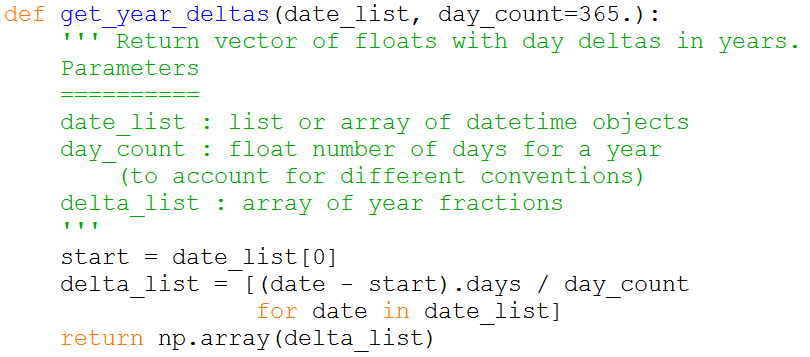
\includegraphics[scale=0.45]{get_year_deltas.png}
\end{figure}
\end{frame}

%------------------------------------------------
\begin{frame}
\frametitle{Modelling and Handling of dates}
An example of using this:
\begin{figure}[H]
	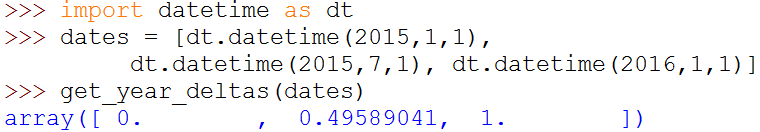
\includegraphics[scale=0.55]{get_year_deltas_example.png}
\end{figure}
\end{frame}

%------------------------------------------------
\begin{frame}
\frametitle{Constant short rate}
\begin{figure}[H]
	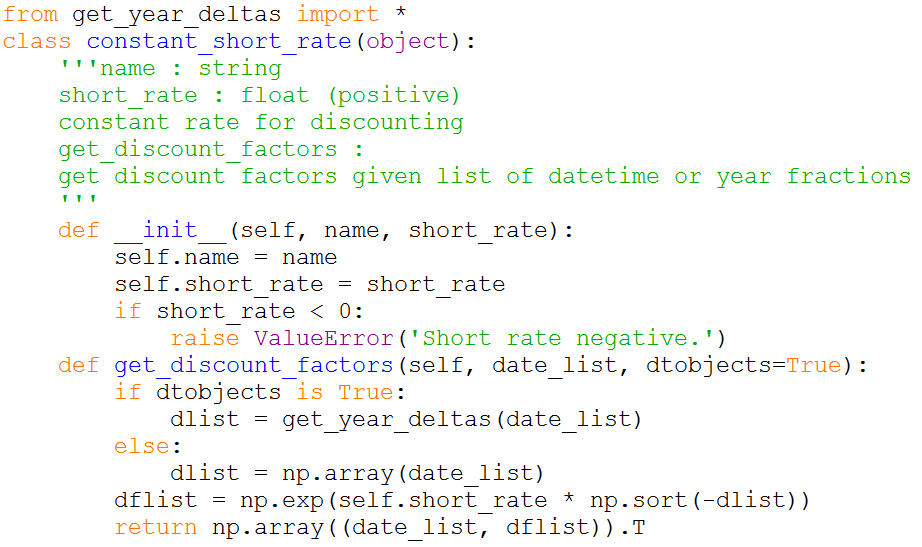
\includegraphics[scale=0.43]{constant_short_rate.png}
\end{figure}
This is a class of constant short rate build only on name and short rate.
Possible extension: maybe we can include the discounting/compounding mechanism as well?
\end{frame}

%------------------------------------------------
\begin{frame}
\frametitle{Constant short rate}
\begin{figure}[H]
	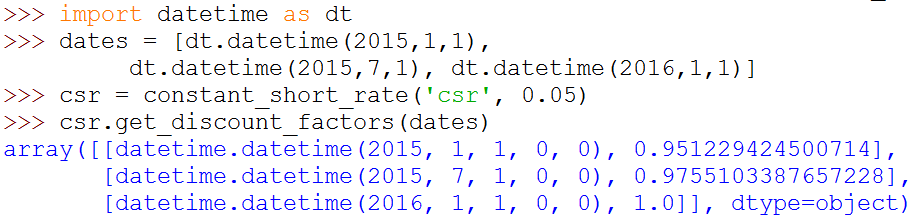
\includegraphics[scale=0.45]{constant_short_rate_example1.png}
\end{figure}
\begin{figure}[H]
	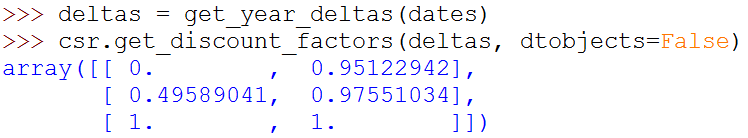
\includegraphics[scale=0.45]{constant_short_rate_example2.png}
\end{figure}
The return value of $get\_discount\_factor$ is a list of pairs of $datetime$ object and corresponding discount factors.
\end{frame}

\subsection{Market environment}
%------------------------------------------------
\begin{frame}
\frametitle{Market environment}
The advantage of using a class as the market environment\\[2mm]
\begin{itemize}
	\item Convenience for consistent modelling
	\item Usage of dictionaries to store constants, lists and curves
	\item Ease of interactions between environments and other objects
	\item Act as a point of integration between previous functions and classes and further developed financial models
\end{itemize}
\end{frame}

%------------------------------------------------
\begin{frame}
\frametitle{Market environment - implementation}
\begin{figure}[H]
	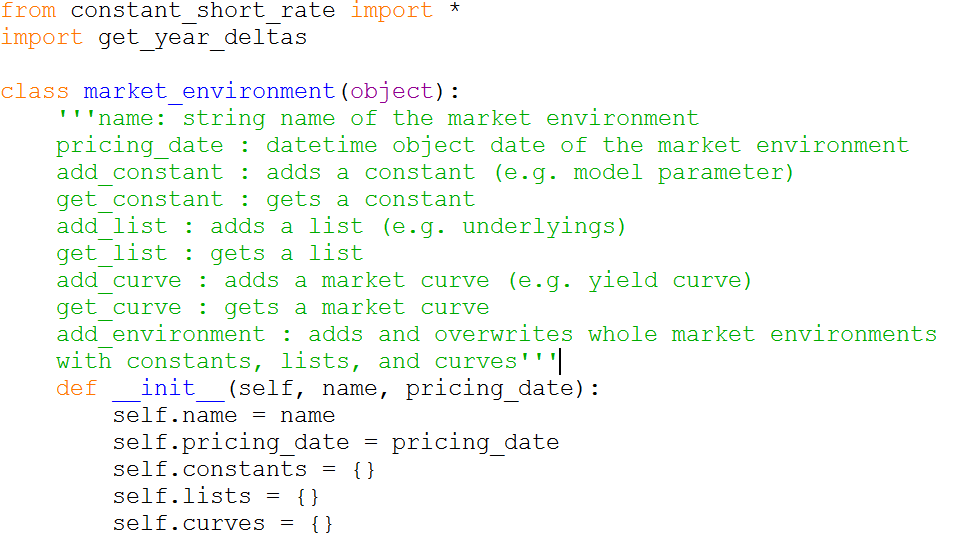
\includegraphics[scale=0.5]{market_environment_1.png}
\end{figure}
\end{frame}

%------------------------------------------------
\begin{frame}
\frametitle{Market environment - implementation}
\begin{figure}[H]
	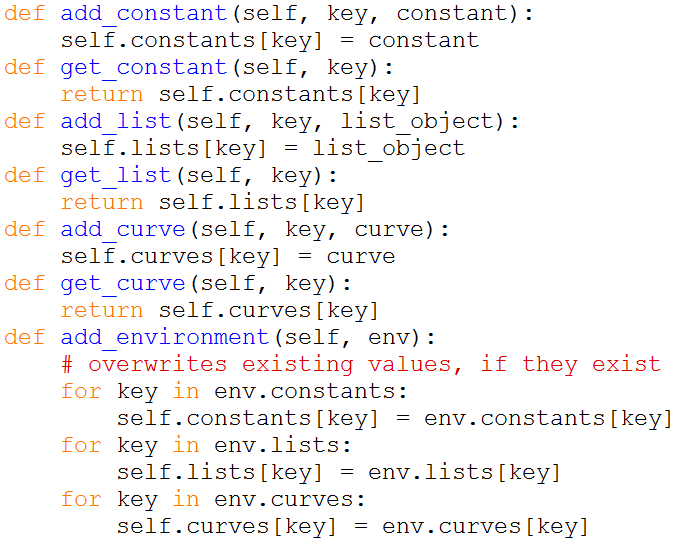
\includegraphics[scale=0.5]{market_environment_2.png}
\end{figure}
\end{frame}

%------------------------------------------------
\begin{frame}
\frametitle{Market environment - testing}
\begin{figure}[H]
	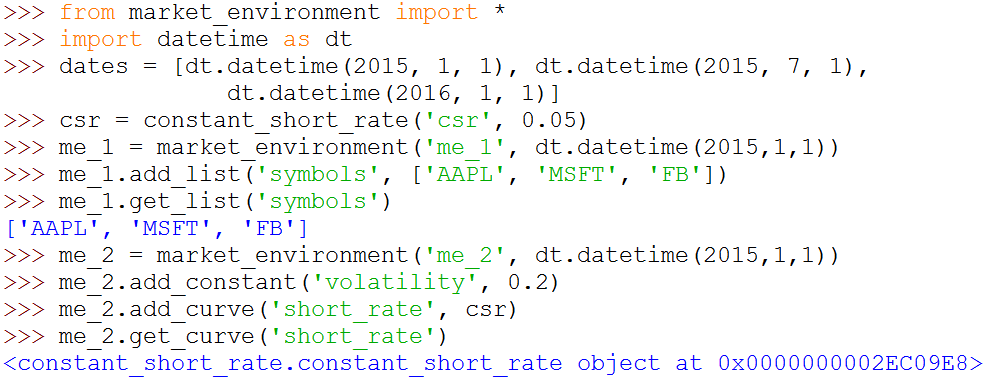
\includegraphics[scale=0.45]{market_environment_example1.png}
\end{figure}
The market environment is able to:
\begin{itemize}
	\item Add/Retrieve list of symbols
	\item Add/Retrieve/Update parameters for the model
	\item Add/Retrieve constant short rate
\end{itemize}
\end{frame}

%------------------------------------------------
\begin{frame}
\frametitle{Market environment - testing}
\begin{figure}[H]
	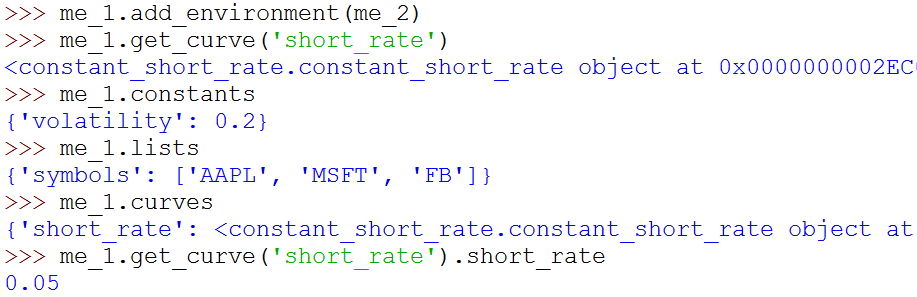
\includegraphics[scale=0.48]{market_environment_example2.png}
\end{figure}
The market environment is able to:
\begin{itemize}
	\item Add all the attributes of another market environment
\end{itemize}
\end{frame}

\subsection{Wrapper class}

%------------------------------------------------
\begin{frame}
\frametitle{Wrapper class - implementation}
\begin{figure}[H]
	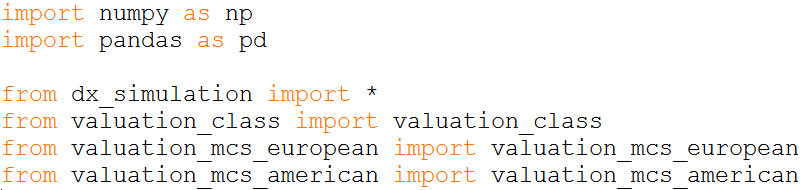
\includegraphics[scale=0.48]{wrapper_class.png}
\end{figure}
With this $dx\_frame.py$, we are now able to import the three components in one line.
\end{frame}

%------------------------------------------------
\begin{frame}
\frametitle{Wrapper class - testing}
\begin{figure}[H]
	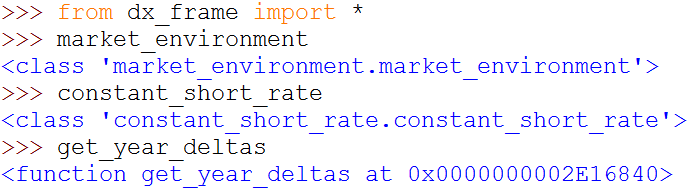
\includegraphics[scale=0.48]{wrapper_class_example.png}
\end{figure}
We are now able to import the entire three components in one line
\end{frame}

%------------------------------------------------
\begin{frame}
\frametitle{Wrapper class - testing}
If we add an $\_\_init\_\_.py$ which has exactly the same content as $dx\_frame.py$ in the same directory, we should be able to directly import like this.
\begin{figure}[H]
	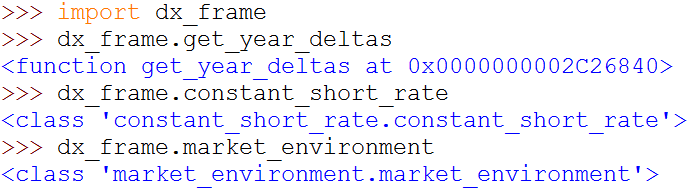
\includegraphics[scale=0.48]{import_wrapper_class_example.png}
\end{figure}
\end{frame}

%-----------------------------------------------
\begin{frame}
\Huge{\centerline{Thank You}}
\begin{center}
\begin{normalsize}
\emph{E0007424@u.nus.edu}
\end{normalsize}
\end{center}
\end{frame}

%------------------------------------------------

\end{document} 